%!TEX program = xelatex
\documentclass[11pt, a4paper]{scrartcl}
%\documentclass[11pt, a4paper]{article}
\usepackage[utf8]{inputenc}
%\usepackage[a4paper,lmargin={3.5cm},rmargin={3.5cm}, tmargin={2.5cm},bmargin = {2.5cm}]{geometry}
\usepackage{setspace}
\usepackage{indentfirst}
\usepackage{mathtools}
\usepackage{enumitem}
\usepackage{graphicx}
\usepackage{yfonts, amsmath, amssymb}
\usepackage[backend=biber, authordate, ibidtracker=context]{biblatex-chicago}
\usepackage{titlesec}
\usepackage{color}
\usepackage{tikz}
\usetikzlibrary{arrows}

\onehalfspacing{}
\addbibresource{conceptsimilarity.bib}

\usepackage{fontspec}
\newfontfamily\osfamily{Latin Modern Roman Demi}

\setkomafont{disposition}{\osfamily}

\renewcommand{\i}[1]{\emph{#1}}
\renewcommand{\L}{\mathcal{L}}
\renewcommand{\v}[1]{\vec{\mathrm{#1}}}
\newcommand{\m}[1]{\textswab{#1}}
\newcommand{\given}[1][]{\:#1\vert\:}

\titleformat{\section}{\Large\bfseries\osfamily}{\thesection}{1em}{}
\titleformat{\subsection}{\large\bfseries\osfamily}{\thesubsection}{1em}{}

\title{\osfamily{}Conceptual Role Semantics \\ in a Spatial Probabilistic Interpretation}
\author{Class Paper for Logic and Probability \\ Prof.\ Dr.\ Hannes Leitgeb \\ SS2017, LMU Munich \\ Conrad Friedrich \\ \texttt{conradfriedrich@posteo.net}}

\begin{document}

\maketitle
\abstract{What can be said about the semantic meaning of a linguistic expression when all that is given is a set of sentences and a subjective probability function, ingredients standardly assumed in formal epistemology? We take a look at several approaches to explicate meaning using spatial metaphors, combining favorable aspects to present an account of similarity in conceptual role based on a spatial interpretation of conditional probabilities.}
\thispagestyle{empty}
\newpage
\tableofcontents
\newpage
\section{Introduction}

With the goal to give a convincing explication of meaning of linguistic expressions by way of mental representation, spatial representations have been used by quite a few authors. In this paper, we start by skimming\footnote{The literature is a bit too vast and deep-reaching for a term paper to firmly put this account in a definite place amongst accounts of meaning, such that the introduction may only serve as a very vague positioning. It would be quite interesting to properly analyze the various theories of mental representation and semantics to see how this account may answer the existing account's objections or assume their merits.} over Gärdenfors' conceptual spaces and Churchland's Semantic State Spaces. To contrast, we summarize Field's account of conceptual role quantified by conditional probabilities. Realizing that Field's notion lends itself to a spatial interpretation, we present an original approach at tying semantics to spaces based on conditional probabilities. We precisify the idea, develop a formal account of conceptual similarity and discuss the consequences of the account when evaluating context-dependent meaning as well as when trying to match inter-speaker meaning to one another. Concluding, we look at salient objections that pop up and create pointers in the direction of future research.\subsection{Gärdenfors' Conceptual Spaces}

Peter Gärdenfors\footnote{Most notably cf. \textcite{gärdenfors2004conceptual} and \textcite{Gardenfors2014-GRDTGO}.} is motivated by results from cognitive science and aims to give a substantial and comprehensive account of mental representation as well as meaning. His account utilizes conceptual spaces to create somewhat of a middle ground between reductivist connectionist and symbolic system approaches to mental representations. The spaces are intended to provide a general framework for presentations. The motivation is, as it strikes me, first and foremost to make sense of descriptive elements. Objects of cognitive experiences get located in spaces made up of dimension determined by qualities belonging to the phenomenal or scientific realm, such as temperature, weight, brightness, pitch and so on. A single object of experience can be located in many such spaces, each making up a domain. There is a specific space for color experience, for example, hue, chromaticness and brightness make up its dimensions. Concepts 

Gärdenfors' Dimensions are rooted in phenomenal experiences and mostly are motivated by empirical, psychological research.

\subsection{Churchland's Semantic State Spaces}


\begin{quote}\singlespacing{} What was presented as new and interesting is therefore something
 quite old and boring, runs the objection. Worse, the emerging ac-
 count leaves unaddressed the question of how each axis of the activa-
 tion space, or each neuron of the representing population, gets its
 semantic or representational content.\footnote{\textcite[7]{10.2307/2564566}}
 \end{quote}

\subsection{Word Space Models in Computational Linguistics}
Its seems like a very natural idea: The geometric interpretation of mental representations provides a promising attempt at an explication of meaning. Geometric approaches have been extraordinarily popular in Computational Linguistics and Natural Language Processing. There, the geometric interpretation or metaphor has a lot of different realisations used for a wide variety of tasks. Quite common is the statistical analysis of huge amounts of data in text form, assigning quantifiable features to linguistic expressions in this data. The goal is to find some statistical patterns in the texts which indicate interesting properties of the linguistic expressions, for example automated recognition of the syntactic role of the expression, or which expressions are named entities, or whether the author of the texts talks about her subject favourably or dismissively. All these tasks have been met with quite the success, suggesting that there is a tangible connection of structural information represented geometrically and what might be generously called the \i{content} of the data. The connection to word meaning is almost straightforward, then, if one takes for example Gärdenfors' instrumentalist position [Citation needed]. Employing a Wittgensteinian functionalist picture of meaning as language \i{use}, the linguist is enabled to research about meaning with computational methods.

What should count as a feature, then, is not trivially determined. Certain distributional properties of expressions present themselves (e.g.\ the frequency of occurring in documents), and it is a feasible approach to use the context of an expression to develop the quantified features. What does that amount to, in practice? Words are counted in texts, and if words are close to one another often, the counts go up. For each expression, this creates something like a co-occurrence profile, which serves as the basis for the spatial representation. Proximity in this representation is then used as an indicator of closeness in meaning. But mere co-occurrence is only a weak indicator for the relation of expressions, their total evidential relations are much more telling. Hence I propose in the following the model similarity of conceptual role through a spatial interpretation of evidential relations between linguistic expressions. 

It's easily answered why computational linguists aren't drawn to the idea of creating a spatial dimensions using conditional probabilities: Since the statistical approaches mentioned earlier use real data and texts, it's safe to say the work is empirical in nature. There is no actual agent's credence function over a natural language to work with, of course, which renders this angle a lot less favorable to the computational linguist. There are, however, theoretical implications which must not necessarily prove useful in the sterilized and idealised philosophical context, on the contrary, it may even enrich the discussion. The practical usefulness of the geometric interpretation is, in my opinion, a hint to its potential theoretical fruitfulness. In other words, I believe that the idealising assumptions made here may take away from the empirical relevance of the present discussion but do not limit any philosophical usefulness.

\subsection{Field's Notion of Conceptual Role}
\subsection{And What That Has to Do With Meaning}

The accounts all say something about meaning, and while I try to avoid to take a stance on the issue, something regarding the nature of meaning has to be said: 

Field seems to adhere to a very traditional extensional explication of meaning, in the sense that the truth conditions for sentences at the actual world seem to play a crucial role in what he calls referential meaning. That is only part of his account, though, and the conceptual role part hints at a more cognitivist aspect of meaning. Conceptual role, as described here, supervenes after all on subjective probabilities, and those are idealisations of mental states. 

Gärdenfors is a proponent of cognitivist semantics, where linguistic expressions refer to something in the mind of the speaker \parencite[154]{gärdenfors2004conceptual}. The association with an external world is then just a matter of pragmatics, and a successfully interacting agent has an appropriate conceptual structure. 

The account used in computational linguistics is mostly functionalist, limiting the meaning of expressions solely to their communicative role. 


\section{Conceptual Similarity in Probabilistic Space}

With this setup, it's a small mental leap to the account of conceptual similarity proposed in this paper. 

Speaking loosely, two sentences are similar in conceptual role if they agree in subjective probability conditional on most sentences, bar a few outliers, or if they mostly agree conditional on all sentences. To make things precise it would be nice to have a \i{distance measure} on conceptual role of sentences (and, possibly, other linguistic entities) relative to a given subjective probability function, not unlike the accuracy measures employed in justification strategies for Bayesianism.\footnote{cf. \textcite{Leitgeb2010}.}

Presupposing subjective probabilities over a language, Field captures sameness in conceptual role (and \i{a fortiori} meaning) of two sentences through comparing their probabilities given each sentence of the language. Yet, the result is only a simple binary categorization. Either two sentences have the exact same conceptual role or they don't. While I find the idea of evidential relations determining the conceptual role of a linguistic expression to be very engaging, it leaves much to be desired. There may be expressions with the same conceptual role in a language, that is for sure, but what about all the other expressions? Don't two sentences with \i{almost} the same conceptual role exhibit an interesting relation to one another? As much has already been deemed plausible by \textcite{Leitgeb2008-LEIAIR}, quoting \textcite{Goodman1949-GOOOLO}. What about whole clusters of expressions? What about the comparison of conceptual roles of sentences between speakers? 

I argue that there is rather interesting information of this type contained in the presupposed subjective probabilities. In this paper, I want to present the general idea, make it somewhat precise and sketch directions for future research.

\begin{figure}
    \centering
\begin{tikzpicture}[x=2cm,y=2cm,z=2cm,>=stealth]
% The axes
    \draw[->] (xyz cs:x=-1.5) -- (xyz cs:x=1.5) node[above] {$\m{c}(\cdot, c_i)$};
\draw[->] (xyz cs:y=-1.5) -- (xyz cs:y=1.5) node[left] {$\m{c}(\cdot, c_j)$};
\draw[->] (xyz cs:z=-1) -- (xyz cs:z=1) node[above] {$\m{c}(\cdot, c_k)$};
% The origin
\node[align=center] at (0.4,-0.2) (ori) {(0,0,0)};
\end{tikzpicture}
\caption{Graphical representation of 3 dimensions of $V$.}
\end{figure}

\subsection{The Central Formalism}\label{sec:central}

Suppose a finite propositional language $\L$ and an agent's subjective probability function $\Pr$ on that language.\footnote{For simplicity, $\L$ here just is a set of sentences.} A spatial representation of the conceptual role of the sentences of the language can be achieved by assigning \i{sentences} to dimensions in a space. Let $V$ be an $n$-dimensional vector space over $\mathbb{R}$, where $n$ is the number of sentences in $\L$. Let's look at a sentence $p \in \L$. To determine its vector in $V$, we measure the \i{evidential relation} of a sentence $c_i$ to $p$ for each dimension, that is, each $c_i \in S$. 

A plausible assumption we adopt from Field is that the evidential relation is captured at least partly by the conditional probability $\Pr(p \given c_i)$, which consequently takes center stage here\footnote{Where defined. Field employs Popper functions in his paper, but since this breaks with the orthodoxy and they mostly prove useful when treating infinite sets \parencite[1352]{Leitgeb2013-LEIRBS}, I assume a classically axiomatised probability function.}. To express the evidential relation in a single number isn't trivial or uncontested (cf. Section~\ref{sec:choosing}), but let's suppose there is such a measure $\m{c}: S \times S \rightarrow \mathbb{R}$. The location of $p$ in the spatial interpretation is then fully determined by $\v{p}~=~(\m{c}({p, c_1}),\dots, \m{c}(p, c_n)) \in V$.

To say something about the relation of the conceptual role of two different sentences $p$ and $q \in \L$, we assume $\v{p}$ and $\v{q} \in V$ and introduce a second measure $\m{d}: V \times V \rightarrow \mathbb{R}^+$ which is intended to measure the distance between $\v{p}$ and $\v{q}$. This can be achieved, among alternatives, by letting ${\m{d}(\v{p}, \v{q})~=~\lVert \v{p} - \v{q} \rVert}$ where 
\[
    \lVert \v{p}-\v{q} \rVert = {\left( \sum_{k=1}^n {(p_k-q_k)}^2 \right)}^{1/2}, 
\]
which is just the euclidean distance. 

The \i{similarity} between two sentences is then just a scoring function that decreases as the distance increases and has a maximum when the distance is minimal, for example: $s_{pq} = e^{-cd_{pq}}$, with a scalar $c$, and where $d_{pq}$ is the distance of two vectors $\v{p}, \v{q} \in V$. 

{\color{red}This is not cleaned up, please write properly.}
In general we have a function ${\m{s}: \mathbb{R}^+ \rightarrow \mathbb{R}^+ }$ that maps distances to similarity measures. We require a monotonically decreasing, continuous function {\color{red} why?}. 

Summing up, we generate a representation of each sentence of the language as a vector in a vector space by measuring its evidential relation to all other sentences of the language with the help of a function $\m{c}$. We then assign similarity scores to pairs of vectors with the composition of distance measure and similarity score: ${\m{s}\circ \m{d} : V \times V \rightarrow \mathbb{R}^+}$.

What is won with this precisification? We now have a precise notion of the spatial interpretation of similarity in conceptual role given an agent's subjective probability function. If we additionally buy into Field's premise of meaning being mainly constituted by conceptual role, the spatial interpretation can tell a lot about the meaning of linguistic expressions. 

For example:

\subsection{Order by Conceptual Similarity}\label{sec:order}

Let's fix a sentence $p$. The spatial structure of the similarity measure induces relations on $\L$ with interesting properties. Perhaps quite obviously, we can define 
\[
    q \leqslant_p r \Leftrightarrow s(p,q) \leqslant s(p,r)
\]
for any two sentences $q$ and $r$, inducing an ordering on $\L$ that is \i{total}, \i{reflexive}, \i{transitive} but \i{not} antisymmetric since two sentences $q$ and $r$ may be equidistant to p, written $q \leqslant_p r$ and $r \leqslant_p q$, while $q \not = r$. Less formally, this relation orders all sentences by conceptual similarity to $p$. Naturally, the most similar sentence to $p$ is $p$ itself, so it holds that for all sentences ${x \in \L}$, ${x\leqslant_p p}$.

Additionally, $\m{s}$ induces equivalence relations on $\L$, so that we can define for sentences $q$ and $r$ 
\[
    q \sim_p r \Leftrightarrow q \leqslant_p r \land r \leqslant_p q,
\]
dividing up all sentences into equidistant equivalence classes relative to $p$.

A neat consequence is another induced ordering: Consider the set of all equivalence classes $\L/\!\sim_p\,=\{ q/\!\sim_p \given q\in \L \}$. We define   
\[
    q/\!\sim_p~\lesssim_p~r/\!\sim_p~\Leftrightarrow q \leqslant_p r, 
\]
and since this is a relation on equivalence classes, the resulting ordering is strict, that is, not reflexive. It is still transitive, however.

Now, let $l_1, \ldots, l_m$ list all elements of $\L/\!\sim_p$ such that $l_i \lesssim_p l_{i+1}$. By definition, we have for $a \in l_i, b \in l_{i+1}$ that $a \leqslant_p b$ for all $0 < i < m$. Geometrically, all elements of $l_i$ are equidistant to $p$ and thus lie on the surface of the same hypersphere. This hypersphere contains all elements of $l_j$ with $j < i$, such that we can define sets $S^1_p, \ldots, S^m_p$ with 
\begin{enumerate}[label = (\roman*)]
    \item $S^1_p = l_1$, with $p \in S^1_p$ and 
    \item\footnote{The inclusion is strict since we already excluded equivalence through the ordering on equivalence classes.}$S^i_p \subset S^{i+1}_p$. 
\end{enumerate}
Or in other words, $S^{i+1}_p \setminus S^{i}_p = l_{i+1}$. See Figure~\ref{fig:spheres} for a graphical representation which shows different levels of similarity to our fixed sentence, $p$. The most similar in conceptual role is $p$ itself.\footnote{Although, of course, there may be distinct sentences with the exact same conceptual role,  such that $S^1_p$ may include additional sentences, which is Field's point.} $S^2_p$ contains all second-closest sentences and so forth. The \i{distance between} two sentences in $S^{i+1}_p\setminus S^{i}_p$ can be greater or less than to $p$, but is limited by the triangle inequality of the metric used.\footnote{$\m{d}(q,r) \leqslant \m{d}(q,p) + \m{d}(r,p)$.} 

\begin{figure}
	\centering
    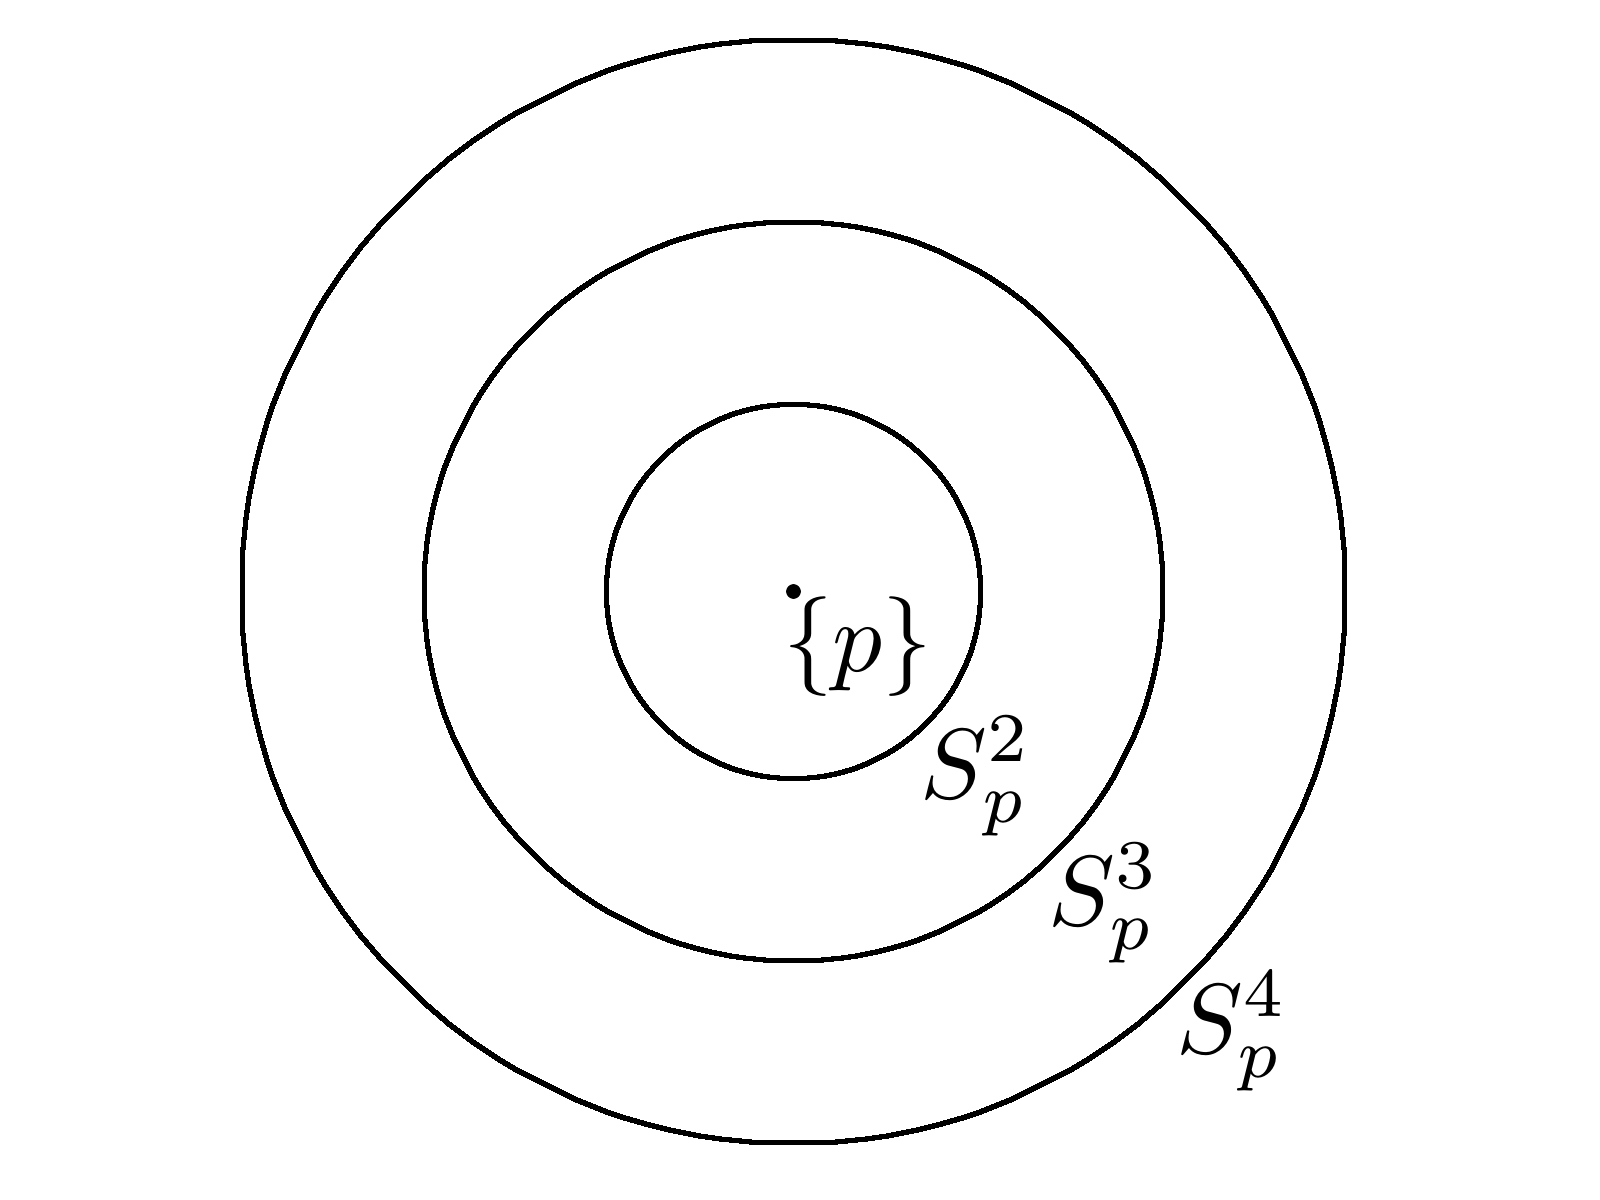
\includegraphics[width=0.75\textwidth]{Similarityspheres.png}
    \caption{A two-dimensional representation of $n$-dimensional conceptual similarity spheres for a simple language with 4 equivalence classes\label{fig:spheres}}
\end{figure}

Since these sets are defined over a conceptual similarity relation (relative to a sentence relative to language and a probability function), these might be called conceptual similarity spheres and bear \i{some} structural resemblance to the similarity spheres used for counterfactual semantics by \textcite{Lewis1973-LEWC-2}, which might already be suspected when glancing at Figure~\ref{fig:spheres}. Most notable differences are that (a) the subjects of discourse here aren't possible worlds at all and instead sentences of a language, that (b) two sentences may inhabit the exact same location, that is, have the same conceptual role, whereas two possible worlds are distinct from one another and (c) that this is not an objective ordering of any kind and instead a purely subjective ordering based on an agent's probability function. Given such a probability function, however, the ordering is rather fix. It would be interesting to investigate under which permutations of different measures the ordering stays invariant.

In short, through some simple structural features, a probability function yields a deep comparative notion of conceptual role of sentences and, one could presume, potentially some insights about meaning.

Next, we'll develop a simple example to see how this notion of conceptual role is applied.

\subsection{A Toy Example: The Lottery}

To use a familiar example, let's consider a standard fair $n$-ticket lottery scenario in which an agents has beliefs about a very narrow set of sentences $\{ t_1, \dots, t_n\}$, where $t_i$ is the sentence that the ticket number $i$ is the winning ticket. Assume a probability distribution of someone who is aware of the real chances involved, i.e.\ that the sentences describe disjoint events, such that $\Pr(t_1) = \cdots = \Pr(t_n) = \frac{1}{n}$ and, more importantly

\[
    \Pr(t_i \given t_j)  =
    \begin{cases*}
        1 & if $i = j$ \\
        0        & otherwise
    \end{cases*}
\]

We might, in this case, set $\m{c}(t_i, t_j) = \Pr(t_i \given t_j)$, set $\v{t_i} = (\m{c}(t_i,t_1),\ldots,\m{c}(t_i,t_n))$, with $\v{t_j}$ accordingly and so with a euclidean distances measure 
\[
    \m{d}(\v{t_i},\v{t_j}) = {\left( \sum_{k=1}^n {(t_{i_k}-t_{j_k})}^2 \right)}^{1/2} = \sqrt{2},  
\]
if $i \not = j$.

Hence, for any fixed $t_i$ there are only two corresponding similarity spheres:\footnote{No matter how we chose the similarity function $\m{s}$, as long as it is monotonously decreasing, as required above.} $S^1_{t_i} = \{ t_i\}$ and $S^2_{t_i}$, which contains all other sentences. 

This result isn't particularly exciting, but it serves well enough to indicate the spatial interpretation of conceptual role: Given no further information, $t_1$ and $t_{10}$ are just as close in meaning as $t_2$ and $t_{77}$. It is easy to see that were we to add additional constraints, such as that you yourself hold the ticket number 25 and we add the sentence $w$: ``I win the lottery!'', the previously strict symmetry is broken and $t_{25}$ takes a spatially distinguished position, since $\Pr(t_{25} \given w) = 1$, but $\Pr(t_l \given w) = 0$ for all other $l$. 

\subsection{Choosing a proper measure}\label{sec:choosing}

As mentioned, choosing the right measure to find what exact quantity gets assigned to the axes of our spatial representation isn't perfectly straightforward. Let's look at such an axis we assign sentence $p$ and $q$, say. Generally, the idea is to use a measure which represents the evidential relation. This is closely related to what is usually called degree of confirmation\footnote{cf. \textcite{Fitelson1999-FITTPO-3}, \textcite{Broessel2013}.}. I'll present to very common measures from Fitelson's extensive discussion: 
\begin{align*}
    \m{c}_d &=_{df} \Pr(p\given q) - \Pr(p)\\
    \m{c}_l &=_{df} \log(\frac{\Pr(p\given q)}{\Pr(p)})
\end{align*}
which both have the desirable properties that
\[
\m{c}_{(\cdot)}(p, q) 
    \begin{cases} 
        > 0 & if \Pr(p \given q) > \Pr(p),\\
        < 0 & if \Pr(p \given q) < \Pr(p),\\
        = 0 & if \Pr(p \given q) = \Pr(p).
    \end{cases}
\]
That is, $\m{c}$ takes a zero value for $\Pr$-independent $p$ and $p$. This makes a spatial representation much more treatable, since irrelevant dimensions just don't have any spatial expansion at all and can be easily disregarded. This were not the case if, for example, we'd just use the conditional probability. The property is highly useful for the account of the next section. 

It is important to note that these two measures aren't ordinally equivalent \parencite[364]{Fitelson1999-FITTPO-3}, meaning that they potentially induce different orderings on $\L$, which is, of course, highly relevant to the present account.

A thorough treatment, then, would include a decision on which measure to use. We're content with mentioning some options and desirable properties for now. 

\section{Context Dependent Conceptual Role}

The whole enterprise of a spatial interpretation of a sentence is somewhat of a holistic approach, in that it evaluates meaning \i{globally} for a fixed language and agent. It is, however, pretty uncontroversial that the lexically same sentence can have different intended meanings, depending on the circumstances of when it's uttered. Relative to different contexts, the same words may mean something different. Can our account accommodate this? 

So far, there has been an implicit assumption that the conceptual role is represented relative to the probability function over the whole language. This needn't be the case, though, and it is mathematically of course perfectly legitimate to restrict the sentences which make up the dimensions of our spatial interpretation. 

\textcite{Stalnaker1978-STAA-2} speaks of common ground amongst speakers in a conversation as establishing a context for utterances. This ground is determined by a context set, which consists in propositions assumed true for the purposes of a particular communication.

In a similar vein, we might adopt the notion of a context set --- populated with sentences instead of propositions --- as a means to restrict the spatial interpretation of conceptual role. Intuitively, this makes some sense: If we ask for a meaning in a particular context, and have already accepted the assumptions about the connection between meaning and evidential relation described in this paper, it is quite natural to restrict the evidential relations that are interesting to us to to those that involve that particular context.

This needn't be just those sentences that correspond to propositions assumed true, but may be extended to sentences deemed \i{relevant} to the current interests. That relevance is commonly spelled out in terms of evidential relation makes determining a context seem circular, at first glance.\footnote{It is not, however. Contexts can be generated from evidential relations through the spatial representation, as well. Since for two sets $C, D \subseteq \L$, $V_{C\cup D}$, $V_{C\cap D}$ and $V_{\L\setminus C}$ are subspaces of $V$, contexts can be combined at will. We ask: Given a sentence $p$, what are relevant other sentences? What could be considered a \i{total} context of $p$? Intuitively those sentences $p$ stands in an evidential relation with, or is not probabilistically independent of. Depending on the measure $\m{c}$ chosen, these are exactly those sentences corresponding to the dimensions $p$ takes a non-zero value in $V$ (cf. Section~\ref{sec:choosing}). This gives a total context set for $p$. Accordingly, this can be generated with additional sentences. The intersection of both total contexts yields the common context.} We assume a context already determined.

Intuitively, then, one way to work with a context is to ``chip away'' at the vector space and remove as many dimensions as needed such that only dimensions corresponding to a context set remain.

More formally, let $V$ be a vector space over $\mathbb{R}$ with dimensions corresponding to sentences in a language $\L$ as above, with an appropriate measure $\m{c}$ chosen. Let $C \subseteq \L$ fix a context set of sentences that interest us, and let $V_C$ be a vector space over $\mathbb{R}$ with dimensions corresponding to sentences in $C$.\footnote{Since $V$ is just $\mathbb{R}^n$, and $V_C$ is just $\mathbb{R}^m$ with $m \leqslant n$, it follows directly that $V_C$ is a subspace of $V$.} Then $V_C$ is a subspace of $V$.

In a subspace like this, the distances between sentences can, of course, change notably compared to the surrounding space, since dimensions that made up the bulk of the distance could be disregarded. Each context, then, induces another family of orderings on $\L$ by conceptual similarity.

The metaphor of a context as a subspace has some interesting advantages. It could be interesting, for example, to compare the change in conceptual role of some expression \i{across} contexts. In what --- quantifiable --- sense is an expression used differently when uttered in another context? If $C$ and $D$ are such context sets, two sentences $p$ and $q \in \L$  (not necessarily in $C$ or $D$) may differ wildly in distance in conceptual similarity given $C$ vs.\ given $D$. 

\section{Inter-Personal Similarity of Conceptual Role}

So far, the spatial interpretation of conceptual role has only been developed for a single language, with a single probability function. What is really interesting, though, is whether the account can be extended so as to include inter-speaker similarity in conceptual role. This is a much needed notion, as it strives to deal with an explication of why communication between two speakers actually works, although they, let's plausibly assume, do not mean \i{exactly} the same when using linguistic expressions. 

The problem is, of course, quite notorious, and we can only hope to hint at a possible solution here.

Intuitively, though, the answer seems clear: two speakers use their expression \i{similarly enough} for communication to properly function, exact sameness in meaning is not required. How does that figure in this account? Can we find a formal explication of this idea? We need to find a measure for the similarity in conceptual role of different speakers. 

In his 1979 paper, Field already probes this problem, and simply gives up:
\begin{quote}\singlespacing{}
  The problem is that different people have different subjective
 conditional probability functions: the machinery developed in this
 paper provides a natural account of what it is for two sentences or
 two terms \i{within the context of the same probability} function to have
 the same conceptual role; but I do not see any way to provide an
 account that is both clear and useful of what it is for terms or sentences in the contexts of \i{different} probability functions to have the
 same role. My own inclination is not to try to provide such an
 account, but the learn to live without the concept of inter-speaker
 synonymy, and all other concepts in terms of which inter-speaker
 synonymy could be defined.\footnote{\textcite[398]{Field1977}, his italics.} 
 \end{quote}

 Field is not explicit about what his reasons are to reject the attainability of a clear and useful account given different probability functions to talk about sameness of conceptual role, but we may suspect that it is for similar reasons as we describe in the following, what we may call the \i{mapping problem} for spatial interpretations of inter-speaker similarity of conceptual role. Of course, Field speaks of \i{sameness} instead of similarity, but since sameness here is just the special case of maximal similarity, we inherit the problems posed for his account.  

\subsection{The Right Mapping Between Languages}

The central problem is how to map the language of one agent to the other agent's language such that pairs of sentences will be assigned to a single dimension in the vector space. That is, when comparing the conceptual role of two sentences of two agents, we need to find a way to represent both languages in the same vector space to make sense of the idea of a distance measure. But which sentences get paired up, as there might not be one-to-one correspondence at all? If just a random sentence is chosen, all information is lost, we instead need to find an pairing that mirrors most closely the \i{structure} of its evidential relations. This challenge can be formalized as follows:

Suppose two speakers with languages $\L$ and $\L'$ and probability functions $\Pr$ and $\Pr'$ over their languages, respectively. The goal is to find a surjective\footnote{We assume here for simplicity of notation that $|\L| \geqslant |\L'|$.} function ${f: \L \rightarrow \L'}$ such that two sentences $p \in \L$ and $p' \in \L'$ can be compared with respect to the measures of evidential relation $\m{c}$ and $\m{c}'$ to other sentences $c_i \in \L$ and $f(c_i) \in \L'$. If we have such a function, a vector for $p$ is determined by $\v{p} = (\m{c}(p,c_i),\ldots,\m{c}(p,c_n))$ as above and for $p'$ by $\v{p}' = (\m{c}'(p',f(c_i)),\ldots,\m{c}'(p',f(c_n)))$. The distance is then calculated as usual: $\m{d}(\v{p},\v{p}')= {( \sum_{i=1}^n {(p_i-p_i')}^2 )}^{1/2}$.  

The simplest case assumes two agents with probability functions over the exact same language. In this case is $\L = \L'$ and the function $f: \L \rightarrow \L'$ is just the identity function, and we are done, it seems like.

But wait a minute: We spoke quite carelessly of identity of sentences so far. What does it mean that $\L = \L'$? The elements are identical. The criterion for sentential identity is lexical identity, such that the sentences ``There are two cats on the mat'' and ``There are 2 cats on the mat'' are \i{not} identical to one another, although they \i{mean} the same, let's assume. On the other hand, two lexically identical sentences may mean something different relative to two agent's probability functions. In fact, two agents may assign wildly different conceptual roles to lexically identical sentences. Using the lexically identical sentences as fixpoints to merge both speaker's spatial representations of conceptual role as described above, then, seems to just beg the question, or at best rely on an empirical assumption that most probably, the lexically same sentence will mean about the same. But this is just what we set out to do: find a measure for semantic similarity. This kind of arbitrariness is unsatisfying for a formal treatment like the one we are undertaking, showing the need for a more general account that, when applied to a case like the simplest one with identical languages, yields in \i{normal} cases just the mapping of sentences to lexically identical ones, while allowing for mappings to other sentences as well, depending on the probability function.{\color{red} CRIES for an example} 

What, then, should determine $f(p)$? Intuitively, the sentence of $\L'$ \i{closest in meaning} to $p$. In normal circumstances, this is quite often the lexically identical sentence, if available. In a general account, this might be any sentence of $\L'$.\footnote{The usefulness of this criterion varies enormously with the commensurability of the languages. If $\L$ is a full-blown no-expenses-spared propositional language akin to a natural language, and $\L'$ is $\{p, q\}$, there is not much sense in asking about semantic similarity across languages. Lets assume somewhat comparable languages.} Isn't this approach even \i{more} question-begging than the last? After all, how are we to quantify semantic similarity if not through the spatial representation? This is a valid concern, however, we need to distinguish between a \i{definition} of $f$, which may be circular, and a \i{criterion} to actually determine $f(c_i)$. The former might not yield an answer to how to do the latter, which might not be a trivial task.

How to define $f$ now? This is just a formalisation of the intuitive idea above. 
We let $\L'$ be $\leqslant_{c_i}$-ordered like in Section~\ref{sec:order}. Then $f(c_i)$ is a maximal element of $\L'$.\footnote{Maximal element because the ordering is not antisymmetric, meaning that there are potentially multiple maximal elements. For this case, we need to chose one. Maybe \i{then} a lexical criterion could be applied, comparing the lexical similarity e.g.\ by taking the Levenshtein-distance.} And that's it. 

To summarize: in order to determine the similarity in conceptual role of two sentences $p$ and $p'$ of different speakers, we calculate the distance $\m{d}(p,p')$, for which we need a mapping $f(c_i) = c_i'$ to determine the terms $\m{c}(p,c_i) - \m{c}(p',c_i')$. To determine $f(c_i)$, we assume $\L'$ to be $\leqslant_{c_i}$-ordered, which just means that we ordered all sentences in $\L'$ by conceptual similarity to $c_i (\in \L)$. In order to do this, we need to calculate the distance $\m{d}(c_i,d')$ for all sentences $d' \in \L'$, for which we need a mapping $f(e_j) = e_j'$ to calculate the terms $\m{c}(c_i,e_j) - \m{c}(d',e_j')$, and so on.

The circularity needn't be a devastating thing, though, as there might exist a recursive algorithm that, given some reasonable assumption, creates a mapping such that the circular definition is satisfied. Such an algorithm is out of the scope of this paper, of course, but since we're already speculating wildly, here is the gist: We build a mapping from the ground up. Assume as a reasonable termination condition some fixpoints of $f$, that is, some such mappings as given. Let's call this set $F \subseteq \L'$. Then, incrementally increase the mappings by adding one sentence $p$ of $\L$ at a time. That is, determine the closest sentence in $\L'$ in the subspace $V_F$. Add that mapping to $F$, and repeat, until every sentence of $\L$ is mapped to $\L'$\footnote{Reasonable constraints apply, of course. It could be, for example, that there isn't a semantically most similar sentence for each sentence in $\L$.}.   

The advantage of this approach is its generality: Let's assume, like we began, the simplest cast of two speakers with $\L = \L'$. If we now assume a normal case, in which most of the lexically identical sentences are closest in conceptual role, too, the whole mapping is easily built. 

The generality extends to more difficult cases, too, and enables us to treat cases of quite dissimilar speaker-languages. The quality of our ``translation'' might drop steadily, though, when the intersection of both languages becomes increasingly small. 

\subsection{A Toy Example: Pastries}

Let's illustrate with a simple example. Assume two speakers, both speaking the same natural language. They share a healthy appetite for a dough-based regional pastry. Their languages are almost lexically identical, let's assume, with the slight contingent difference that speaker $\alpha$ refers to the pastry as `Berliner' while speaker $\alpha'$ never even heard of the term and uses `Krapfen' instead. Let's call the intersection of both languages $\L \cap \L' = F$ and generously assume lexically identical sentences to also be semantically most similar, as described above. Consequently, every element of $\L\setminus \L'$ has the word `Berliner' in it, and `Krapfen' \i{vice versa}.

With this setup, we try and find the semantically most similar sentence of $\L'$ to $s =$ `Ich mag Berliner!' of $\L$. According to the definition, we ought to find the maximal element of $\L$ under $\leqslant_s$, for which we need to calculate $\m{d}(\v{s},\v{l'})$ for each $l' \in \L'$. But we can't --- there is no mapping for $\L\setminus\L'$. There is one, however, for $F$ --- the identity function. We now can approximate the most similar element of $\L'\setminus\L$ to each element of $\L\setminus\L'$ by using the subspace $V_F$, expanding the subspace in each iteration to include an axis for the element added in the previous iteration. At last, unsurprisingly, we determine the closest element to `Ich mag Berliner!' as `Ich mag Krapfen!'. 

\section{Conclusions, Objections, and Future Research}

Symmetry (contexts help here) and Transitivity can be problematic, see Gardenfors 2004 p. 112 and Lewis (p. 51)

Maybe problems with indexical expressions? Could be better to define the whole schose on possible worlds instead\ldots

p and q can be on the same semantic location but be different sentences

\textcite{Leitgeb2008-LEIAIR} constructs an impossibility result for the very concept of meaning similarity, concluding that either its doomed or we'd have to give up a substantial bit of compositionality. Although I haven't said naught about compositionality, it's still a feature that shouldn't be disregarded, of course. To make Leitgeb's result work, we (i) must make sense of our account in terms of a binary relation: Sentences $p$ and $q$ can be meaning similar, period. To accommodate this, we could introduce a threshold $\epsilon$ under which two meanings are similar. And we (ii) need to expand the account on countably infinite languages. And we (iii) need to assume connectedness of meaning similarity, which means that for two sentences $p$ and $q$ there is a chain of meaning similarity-connected sentences starting with $p$ and ending with $q$. To \i{avoid} the result, we could, apart from simply denying (i) or (ii), argue that connectedness does not hold in general.Since our space is sparse with as many vectors as dimensions, distances between vectors may be such that there are clusters of sentences, without distances less than $\epsilon$ to the next cluster for any element.

Linguistic Entities

Conceptual Learning

Churchland structural similarity for inter-speaker meaning

It might raise a few suspicions to use a normative epistemological concept, rational degree of belief in form of a subjective probability function, to explicate semantic meaning. In particular, it is not clear if the resulting account is normative. Is this now
\section{Replace Meaning with Conceptual Role}
%\nocite{*}
\begin{singlespacing}
\printbibliography{}
\end{singlespacing}
\end{document}
